\documentclass[aspectratio=169,10pt,t]{beamer}
% \usetheme[
% %%% options passed to the outer theme
% %    progressstyle=fixedCircCnt,   %either fixedCircCnt, movCircCnt, or corner
% %    rotationcw,          % change the rotation direction from counter-clockwise to clockwise
% %    shownavsym          % show the navigation symbols
%   ]{SDUsimple}
\usepackage{SDUtheme/beamerthemeSDUsimple}
% If you want to change the colors of the various elements in the theme, edit and uncomment the following lines
% Change the bar and sidebar colors:
%\setbeamercolor{SDUsimple}{fg=red!20,bg=red}
%\setbeamercolor{sidebar}{bg=red!20}
% Change the color of the structural elements:
%\setbeamercolor{structure}{fg=red}
% Change the frame title text color:
%\setbeamercolor{frametitle}{fg=blue}
% Change the normal text color background:
%\setbeamercolor{normal text}{fg=black,bg=gray!10}
% ... and you can of course change a lot more - see the beamer user manual.
\usepackage{color}
\usepackage{float}
\usepackage{dsfont}                         % Enables double stroke fonts
\usepackage{bm}
\usepackage[utf8]{inputenc}
\usepackage[english]{babel}
\usepackage[T1]{fontenc}
\usepackage{listings}
\usepackage{amsmath}
\usepackage{booktabs}
\usepackage{import}
% Or whatever. Note that the encoding and the font should match. If T1
% does not look nice, try deleting the line with the fontenc.
\usepackage{helvet}
\usefonttheme{professionalfonts}

\newtheorem{algorithm}{Algorithm}
%\newtheorem{problem}{Problem}
\newtheorem{proposition}{Proposition}
% colored hyperlinks
\newcommand{\chref}[2]{%
	\href{#1}{{\usebeamercolor[bg]{SDUsimple}#2}}%
}

\title{Grouping and Clustering}
\subtitle{Multivariate Statistic}
%\date{\today}
\date{ }

\author{
	Made by: \\
	\textbf{Lasse Gøransson, Marc Evald, Anne-Charlotte Poulsen \& Aske Møller}
}

% - Give the names in the same order as they appear in the paper.
% - Use the \inst{?} command only if the authors have different
%   affiliation. See the beamer manual for an example

\institute[
%  {\includegraphics[scale=0.2]{SDU_segl}}\\ %insert a company, department or university logo
SDU Robotics\\
The Maersk Mc-Kinney Moller Institute\\
University of Southern Denmark
] % optional - is placed in the bottom of the sidebar on every slide
{% is placed on the bottom of the title page
	SDU Robotics\\
	The Maersk Mc-Kinney Moller Institute\\
	University of Southern Denmark

	%there must be an empty line above this line - otherwise some unwanted space is added between the university and the country (I do not know why;( )
}

% specify a logo on the titlepage (you can specify additional logos an include them in
% institute command below
\pgfdeclareimage[height=0.5cm]{titlepagelogo}{SDUgraphics/SDU_logo_new} % placed on the title page
%\pgfdeclareimage[height=1.5cm]{titlepagelogo2}{SDUgraphics/SDU_logo_new} % placed on the title page
\titlegraphic{% is placed on the bottom of the title page
	\pgfuseimage{titlepagelogo}
	%  \hspace{1cm}\pgfuseimage{titlepagelogo2}
}

\begin{document}
% the titlepage
{\SDUwavesbg%
	\begin{frame}[plain,noframenumbering] % the plain option removes the header from the title page
		\titlepage
\end{frame}}
%%%%%%%%%%%%%%%%


\begin{frame}[t]
	\frametitle{Agenda}

	\begin{itemize}
		\item Motivation
		\item Distance Measure
		\item Search Methods
			\begin{itemize}
				\item Hierarchical Grouping
				\item K-Means Clustering
				\item Gaussian Mixture
			\end{itemize}
	\end{itemize}

\end{frame}

\begin{frame}[t]
	\frametitle{Motivation}

	Split observation into K clusters

\end{frame}

\begin{frame}[t]
	\frametitle{Distance Measure}
	\framesubtitle{Between Observations}

	\begin{columns}
		\begin{column}{0.3\textwidth}

			Properties

		\end{column}
		\begin{column}{0.5\textwidth}

			\[
				\begin{aligned}
					d \left( x ,y  \right) 
			&=
			\left( 
				\sum^{p}_{i=1} | x_i - y_i | ^{m}
			\right) ^{ \frac{1}{m} }
			\\
			d \left( x ,y  \right) 
			&=
			\sqrt{
				\sum^{p}_{i=1}  \left(  x_i - y_i  \right)  ^{2}
			}
			d \left( x ,y  \right) 
			\\
			d \left( x,y \right) 
			&=
			\sum^{p}_{i=1}  | x_i - y_i |
				\end{aligned}
			.\] 

		\end{column}
	\end{columns}


\end{frame}

\begin{frame}[t]
	\frametitle{Distance Measure}
	\framesubtitle{Between Clusters}

	\begin{figure}[h]
		\centering
		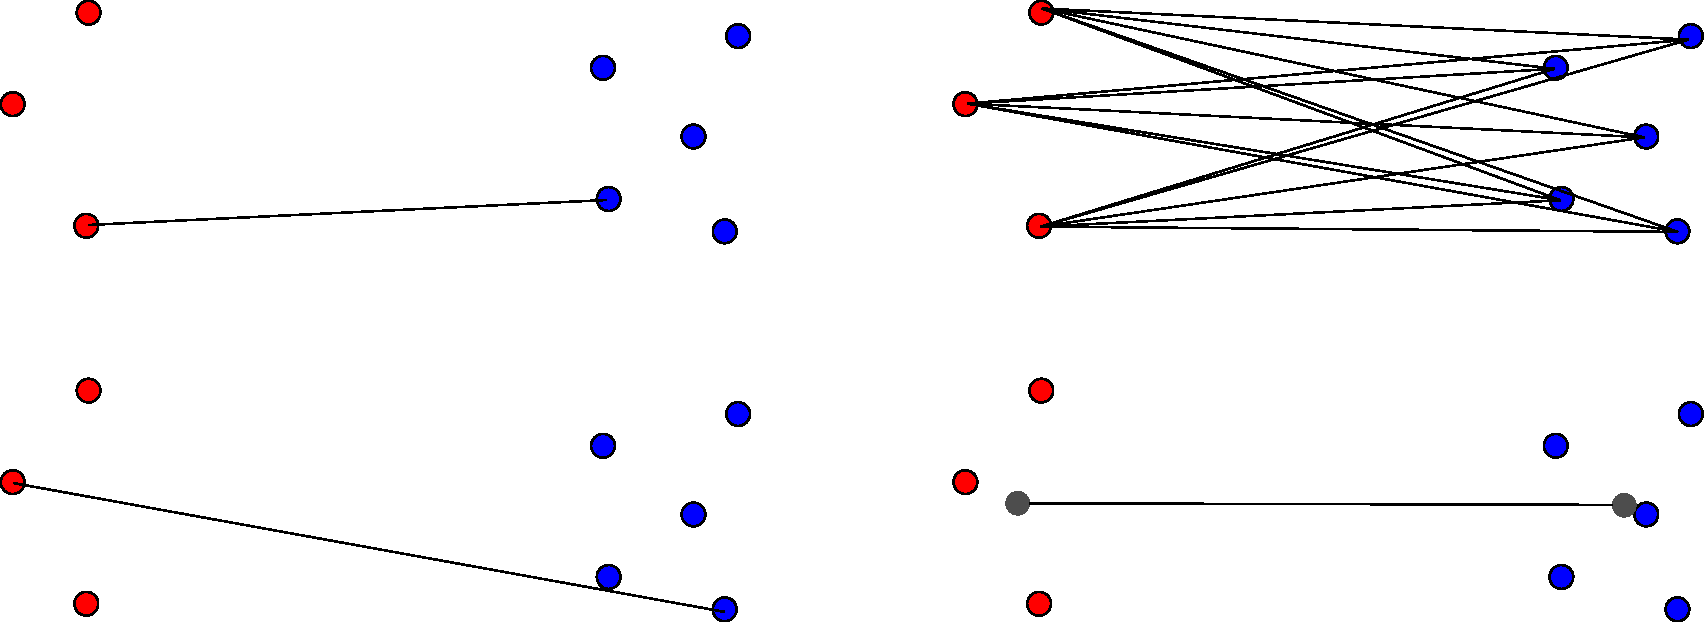
\includegraphics[width=\textwidth]{images/linkage.pdf}
	\end{figure}
\end{frame}


\begin{frame}[t]
	\frametitle{Search Methods}
	\framesubtitle{Hierarchical}

	\begin{columns}
		\begin{column}{0.5\textwidth}
			\[
				D = \begin{bmatrix}
					0 & d_{12} & \cdots & d_{1n}\\
						& \ddots & & \\
						&& \ddots& \\
						&&&0
				\end{bmatrix}
			.\] 
		\end{column}
		\begin{column}{0.5\textwidth}

			\begin{figure}[h]
				\centering
				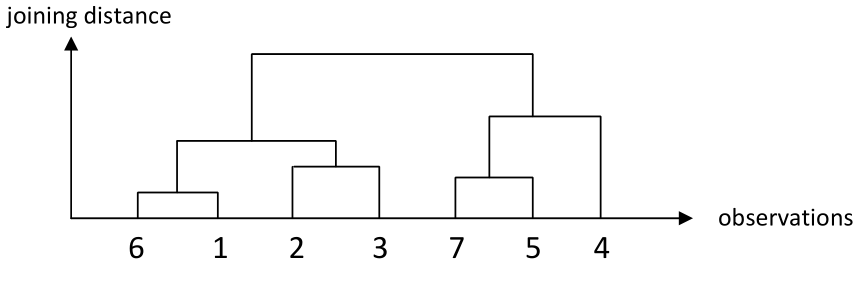
\includegraphics[width=1\textwidth]{images/hirakisk-2.png}
			\end{figure}
		\end{column}
	\end{columns}
\end{frame}

\begin{frame}[t]
	\frametitle{Search Methods}
	\framesubtitle{K-means}

	\begin{figure}[h]
		\centering
		\scalebox{0.7}{
			\import{images/}{k-means.pdf_tex}
		}
	\end{figure}

\end{frame}

\begin{frame}[t]
	\frametitle{Search Methods}
	\framesubtitle{Gaussian Mixture}


	\begin{itemize}
		\item Model\\
			\[
				f _{X} \left( X \right)  =
				\sum^{K}_{k=1} 
				p_k f _{Y_k}  \left( x \right) ,
				\hspace{1cm}
				x = \left[ x_1, \cdots, x_p \right] ^{T}
			.\] 
			\pause
		\item Estimate 
			\[
				L  \left( \{ p_k \} ^{K}_{k=1},
					\{ \mu_k \}^{K}_{k=1},
					\{ \Sigma_{k} \}^{K}_{k=1}
				\right) 
			.\] 
			\pause
		\item Evaluation
			\[
				\begin{aligned}
					AIC &= 2 \log L _{\max} - 2
					\left( K \cdot  \left[ 1 + \frac{p \left( p+3 \right) }{2}  \right] -1  \right) \\
					BIC &= 2 \log L _{\max} -
					\left(  K \cdot  \left[ 1 + \frac{p \left( p+3 \right) }{2}  \right] -1  \right) 
					\log n
				\end{aligned}
			.\] 
    \item Assign Clusters
	\end{itemize}


\end{frame}

\begin{frame}[t]
	\frametitle{Search Methods}
	\framesubtitle{Gaussian Mixture}
    
	\begin{figure}[h]
		\centering
		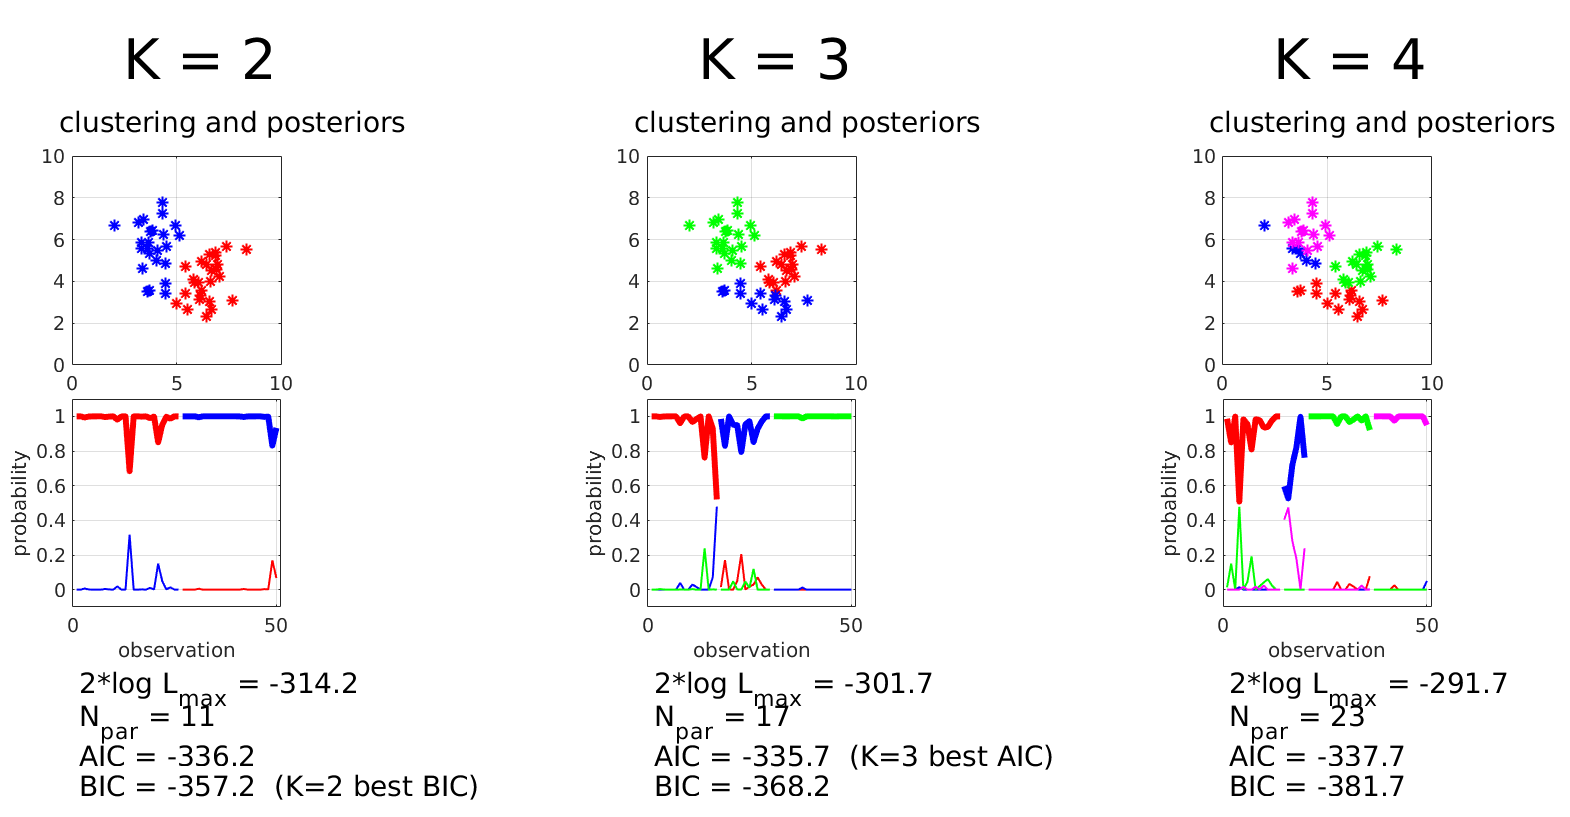
\includegraphics[width=0.8\linewidth]{images/gmm.png}
	\end{figure}

\end{frame}

\end{document}
